\section{A formal foundation for brushing and linking}
\label{sec:toolkit}

Intuitively, selections in outputs computed from the same data can be linked through their common data dependencies, which also has a bidirectional quality: one must consider how dependencies flow ``backward'' from selections in one chart to a selection $S$ in the underlying data, and then ``forward'' from the selected data $S$ to a corresponding selection in the other chart. However, the flavour of the forward dependency differs from the notion of ``sufficiency'' outlined in the previous section: to determine the related parts of the other chart, we must consider not what the data selection $S$ is \emph{sufficient} for, but what it is \emph{necessary} for: those parts of the other visualisation that depend on $S$. In particular, the forward dependency is not simply the upper adjoint $\evalFwdF{T}$ of the dependency relation $\evalBwdF{T}$. We now show how the idea of the \emph{complement} of a selection can be used to derive such a relation from the analysis given in \secref{data-dependencies}. We also contrast the approach presented in this paper with prior work on program slicing based on Galois connections.

\begin{figure}
   \begin{subfigure}{0.53\textwidth}
      {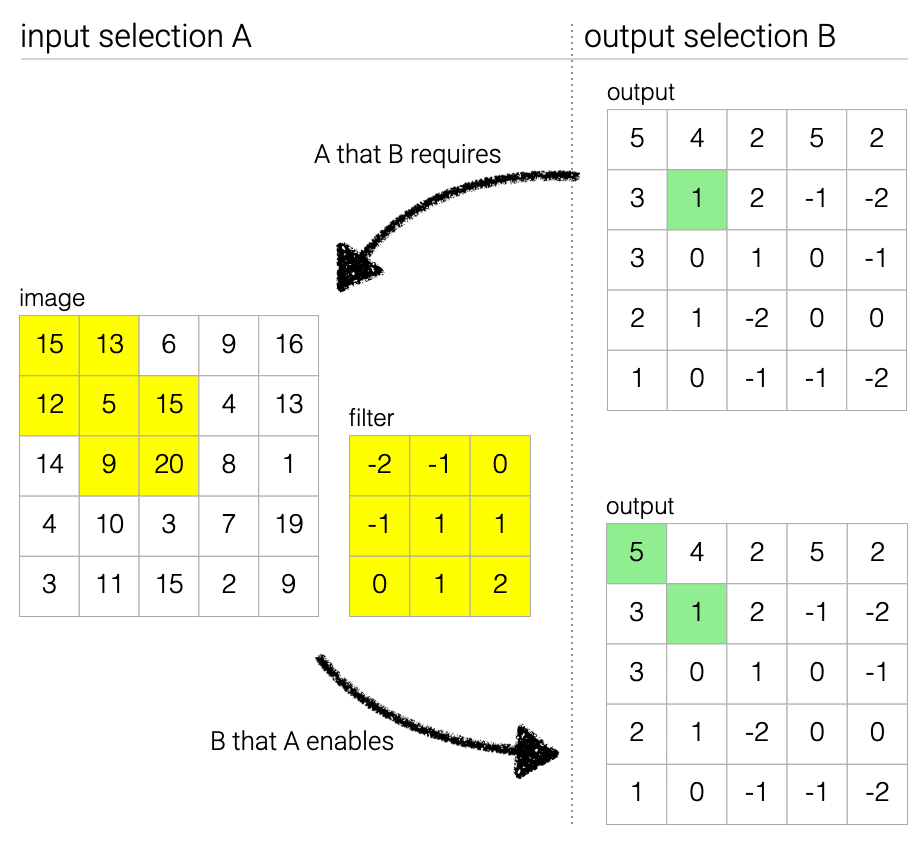
\includegraphics[scale=0.4]{fig/example/4-relations-1.png}}
      \vspace{2mm}
      \caption{Galois dependency $(\evalBwdF{T}, \evalFwdF{T})$}
      \label{fig:example:convolve-viz:galois-dependency}
   \end{subfigure}
   \begin{subfigure}{0.46\textwidth}
      {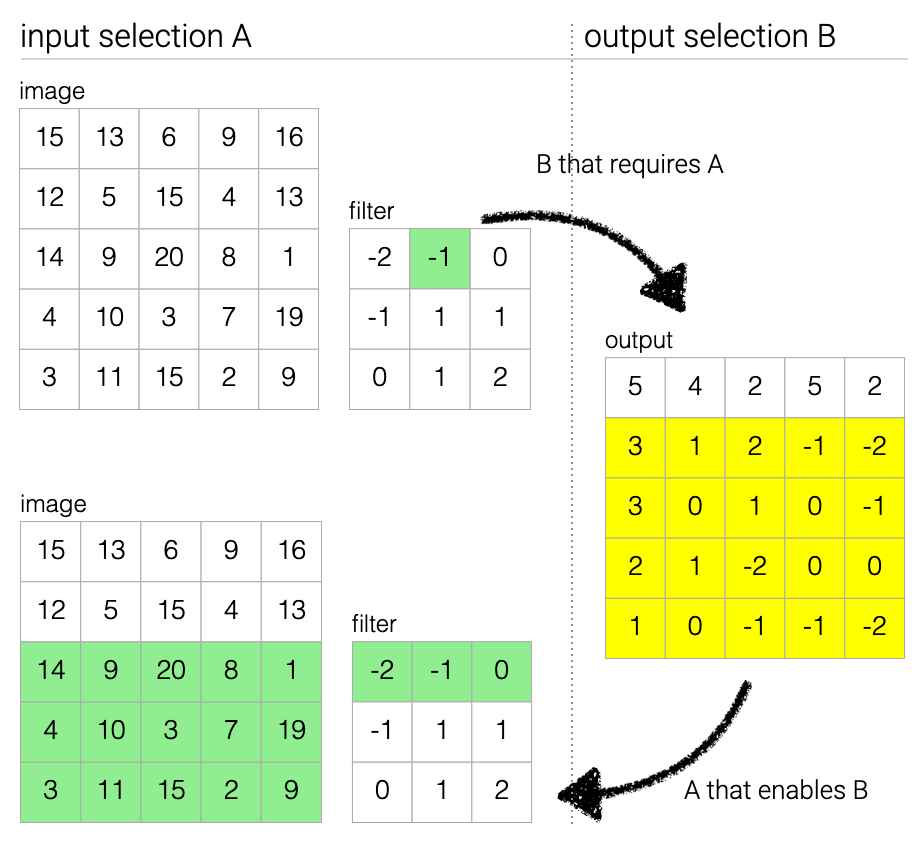
\includegraphics[scale=0.4]{fig/example/4-relations-2.png}}
      \vspace{2mm}
      \caption{De Morgan dual $(\dual{\evalFwdF{T}}, \dual{\evalBwdF{T}})$}
      \label{fig:example:convolve-viz:de-morgan-dual}
   \end{subfigure}
   \caption{Upper and lower pairs are dual; left and right pairs are adjoint}
   \label{fig:example:convolve-viz}
\end{figure}


\subsection{Linking cognate visualisations}

We call two outputs \emph{cognate} if they are computed from common data.

\todo{Introduce negation and the other Galois connection that can be derived from negation.}

\subsection{Relationship to Galois slicing}

in the program slicing literature, dynamic analyses based on Galois connections have been developed for pure functional programs~\cite{perera12a}, functional programs with effects~\cite{ricciotti17}, and \piCalculus~\cite{perera16d}. These ``Galois slicing'' techniques have the flavour of what we need, but are unable to compute the kind of sufficiency relation we just outlined. To see the problem, we briefly outline how Galois slicing works. The idea is generalise the notion of program and value to \emph{program slices} and \emph{value slices}, program and values where some subexpressions have been replaced by hole $\hole$. A program slice ``evaluates'' to a \emph{value slice}, a value where some subvalues have been replaced by $\hole$, and dual to this, a value slice induces a (minimal) program slice. One can then extend this basic framework to focus on

The problem with this approach is that it does not readily extend to a notion of selection where the part of the output of interest is not a prefix of the output, but rather a prefix of some subtree. For example, if we consider the following program, which has the value \lstinline{(0.4, 0.6)}:

\begin{figure}
   \small
   \begin{centering}
      \begin{subfigure}{0.45\textwidth}
         {\lstinputlisting[language=Fluid,escapeinside={(*@}{@*)}]{other-src/diff-slicing-0.example}}
      \caption{Original program}
      \label{fig:example:diff-slicing:original}
      \end{subfigure}
      \begin{subfigure}{0.45\textwidth}
         {\lstinputlisting[language=Fluid,escapeinside={(*@}{@*)}]{other-src/diff-slicing-2.example}}
      \caption{Backward slice for \kw{(0.4, $\hole$)}}
      \label{fig:example:diff-slicing:subtree}
      \end{subfigure}
      \\
      \begin{subfigure}{0.45\textwidth}
         {\lstinputlisting[language=Fluid,escapeinside={(*@}{@*)}]{other-src/diff-slicing-1.example}}
      \caption{Backward slice for spine \kw{($\hole$, $\hole$)}}
      \label{fig:example:diff-slicing:spine}
      \end{subfigure}
      \begin{subfigure}{0.45\textwidth}
         {\lstinputlisting[language=Fluid,escapeinside={(*@}{@*)}]{other-src/diff-slicing-3.example}}
      \caption{Differential backward slice for \kw{(\codeSelTwo{0.4}, $\hole$)}}
      \label{fig:example:diff-slicing:differential}
      \end{subfigure}
   \end{centering}
   \vspace{-2mm}
   \caption{Differential Galois slicing selects input (blue) needed \emph{only} for selected output (green)}
   \label{fig:example:diff-slicing}
\end{figure}


\noindent Because differential slicing includes a program part if is needed \emph{only} by the selected output, in general it underapproximates the parts actually needed for the selected output. In this example, \lstinline{2} and \lstinline{3} are both needed to compute the spine containing the subtree of interest, and so the differential slice does not include them. Differential slicing based on tree prefixes is thus not a suitable technique for computing data dependencies.

Our approach does have one disadvantage vis-\'a-vis Galois slicing, namely that a program ``selection'' does not really resemble a program, but merely picks out various constants and constructors in the program involved in constructing the output selection. With Galois slicing, the program slice is a program with some holes. Although it is not executable as-is, one could (for example) imagine replacing holes by arbitrary expressions of an appropriate type, in order to recover an executable slice. It is not clear with our approach how to ``extract'' an executable slice for a particular output selection; for primitive values, one could extract the \emph{expression provenance} \cite{acar12}, which would explain how the primitive value was computed using primitive operations, but it is not easy to see how this generalises to structured outputs. Moreover there is no property that ensures the expression provenance is in some sense a projection of the semantics of the original program; \cite{field98} explore this notion of executable slice in the context of term rewriting systems, so perhaps this idea could be adapted to our core calculus and used to derive a notion of execution slice. \todo{Needs work -- perhaps move this paragraph to Related work.}
